\section{Composition}\label{sec:composition}

Throughout this section $A=\lay SD$ is a layout with values in $\D$, with scales
$P_1,\dots,P_{m-1}$ and jumps $\jump_1,\dots,\jump_{m-1}$, and
$B=\lay{(t_0,\dots,t_{n-1})}{(r_0,\dots,r_{n-1})}$ is an $\N$-valued layout with shape $T$. We
write
\[ g=\ext A\circ\bnd B\colon\ \rng{|T|}\to\D \]
for the honest composite function, and identify $x\in\rng{|T|}$ with its digit vector
$c=(c_0,\dots,c_{n-1})\in\rng{t_0}\times\dots\times\rng{t_{n-1}}$, so that
$\bnd B(x)=\sum_jc_jr_j$.

\subsection{What a composite must be}

CuTe asks for a layout $R$ with $B\preceq R$ and $R(c)=A(B(c))$. For flat $B$ the condition
$B\preceq R$ says that $R=(R_0,\dots,R_{n-1})$ with $|R_j|=t_j$: every mode of $B$ may be
subdivided, but not merged with its neighbours.

\begin{definition}\label{def:composition}
A \emph{by-mode refinement} of $T$ is a shape $T'=T'_0T'_1\cdots T'_{n-1}$ (concatenation) with
$|T'_j|=t_j$; then $B'=\lay{T'}{R'}$, in which the stride of each non-unit mode is the value of
$\bnd B$ at the corresponding unit of $T'$ (and unit modes have stride $0$), has the same function
as $B$ and is called a by-mode refinement of $B$. We say that
\emph{$A\circ B$ exists} if $g$ is $T'$-additive for some by-mode refinement $T'$ of $T$.
\end{definition}

\begin{lemma}[the composite is forced; case $T'=T$\mech]\label{lem:forced}
If $g$ is $T'$-additive, then $g=\bnd{\lay{T'}{D'}}$ where the stride of each non-unit mode is the
value of $g$ at the corresponding unit; for $T'=T$ this is $d'_j=\ext A(r_j)$. Moreover, if
$R=(R_0,\dots,R_{n-1})$ is a composite then $\bnd{R_j}(x)=\ext A(r_jx)$ for $x\in\rng{t_j}$.
Hence $A\circ B$, if it exists, is unique up to the choice of the refinement, and unique once each
$R_j$ is required to be coalesced.
\end{lemma}
\begin{proof}
The first claim is \cref{prop:additive}. For the second, apply \cref{prop:concat} to $R$ and to
$B$ with all coordinates but the $j$-th equal to zero.
\end{proof}

\noindent So there is nothing to choose: \emph{composing with $B$ means evaluating $A$ at the
strides of $B$}. The only question is whether the result has the right function.

\subsection{Evaluation plus carry defect}

\begin{theorem}[composition formula\mech]\label{thm:defect}
For every $c\in\rng{t_0}\times\dots\times\rng{t_{n-1}}$,
\begin{equation}\label{eq:defect}
 \ext A\Bigl(\sum_jc_jr_j\Bigr)=\sum_{j=0}^{n-1}c_j\cdot\ext A(r_j)\;+\;\sum_{i=1}^{m-1}\Cdef_i(c)\cdot\jump_i,
\qquad
 \Cdef_i(c)=\floor{\frac{\sum_jc_j\,(r_j\bmod P_i)}{P_i}} .
\end{equation}
\end{theorem}
\begin{proof}
$\sum_jc_jr_j$ is a sum of $\sum_jc_j$ numbers, $r_j$ occurring $c_j$ times. Apply
\cref{thm:carry}; the carry count~\eqref{eq:carrycount} at scale $P_i$ is $\Cdef_i(c)$.
\end{proof}

The first term on the right is the function of the \emph{naive composite}
$\lay{T}{(\ext A(r_0),\dots,\ext A(r_{n-1}))}$; the second term, the \emph{carry defect}, counts
the carries that occur in $A$'s radix when $\sum_jc_jr_j$ is evaluated by the schoolbook
method, each weighted by the jump of $A$ at that scale.

\begin{corollary}[\mech]\label{cor:naive}
The naive composite has function $g$ if and only if $\sum_i\Cdef_i(c)\cdot\jump_i=0$ for all $c$.
\end{corollary}

\begin{theorem}[exact composability]\label{thm:exact}
The following are equivalent.
\begin{enumerate}[label=(\roman*),itemsep=1pt]
\item $A\circ B$ exists.
\item Some by-mode refinement $B'$ of $B$ has vanishing carry defect against $A$.
\item For each $j$, the function $x\mapsto\ext A(r_jx)$ on $\rng{t_j}$ is a layout function, and
 $\ext A\bigl(\sum_jy_j\bigr)=\sum_j\ext A(y_j)$ whenever $y_j\in\{0,r_j,\dots,(t_j-1)r_j\}$ for all $j$.
\item $g$ is a layout function and $\spec(g)\cup\Sc(T)$ is a chain under divisibility.
\end{enumerate}
If they hold, $A\circ B=(R_0,\dots,R_{n-1})$, where $R_j$ is the coalesced layout of
$x\mapsto\ext A(r_jx)$.
\end{theorem}
\begin{proof}
(i)$\Leftrightarrow$(ii): by \cref{lem:forced} a composite over $T'$ is the naive composite of $A$
and $B'$; apply \cref{cor:naive} to $B'$.
(i)$\Leftrightarrow$(iv): by \cref{thm:spectrum}, $g$ is $T'$-additive iff
$\spec(g)\subseteq\Sc(T')$. The sets $\Sc(T')$, for $T'$ a by-mode refinement of $T$, are exactly
the chains of divisors of $|T|$ in $\{2,\dots,|T|-1\}$ that contain $\Sc(T)$. So a suitable $T'$
exists iff $\spec(g)\cup\Sc(T)\cup\{|T|\}$ is a chain under divisibility, that is, iff $g$ is a
layout function (\cref{thm:spectrum}(a)) and $\spec(g)\cup\Sc(T)$ is a chain.
(i)$\Rightarrow$(iii): if $R=(R_0,\dots,R_{n-1})$ is a composite, then $x\mapsto\ext A(r_jx)$ is
the function of $R_j$ (\cref{lem:forced}), and \cref{prop:concat} applied to $R$ gives
$\ext A(\sum_jr_jc_j)=\sum_j\bnd{R_j}(c_j)=\sum_j\ext A(r_jc_j)$.
(iii)$\Rightarrow$(i): let $R_j$ be a layout with function $x\mapsto\ext A(r_jx)$; by
\cref{prop:concat} the layout $(R_0,\dots,R_{n-1})$ has function
$c\mapsto\sum_j\ext A(r_jc_j)=\ext A(\sum_jr_jc_j)=g(c)$.
\end{proof}

Condition (iii) separates two issues: each mode of $B$ must be composable on its own, and the
modes must not \emph{interfere}. By \cref{thm:carry}, interference is again a matter of carries:
the second half of (iii) says that the carries produced when the $n$ numbers $r_jc_j$ are added
are invisible to $A$. Both requirements of (iv) are needed. For $A=(2,3):(0,1)$ and
$B=(3,2):(1,3)$ the composite $g=(0,0,1,1,2,2)$ is a layout function with $\spec(g)=\{2\}$, but
$2$ is not comparable with the scale $3$ of $T$, and $A\circ B$ does not exist (whereas
$A\circ(6:1)=(2,3):(0,1)$ does). For $A=(2,2):(1,3)$ and $B=3:1$ we get $g=(0,1,3)$ with
$\spec(g)=\{2\}$, a chain; but $2\nmid3$, so $g$ is not a layout function.

\subsection{The carry-free criterion}

\begin{definition}\label{def:carryfree}
$B$ is \emph{carry-free at scale $P$} if $\sum_j(t_j-1)\,(r_j\bmod P)<P$. $A$ has
\emph{independent jumps} if $\sum_in_i\cdot\jump_i=0$ with all $n_i\in\N$ implies $n_i=0$ for
every $i$ with $\jump_i\neq0$.
\end{definition}
\noindent Being carry-free at $P_i$ means $\Cdef_i\equiv0$, because $\Cdef_i$ is largest at
$c=(t_0-1,\dots,t_{n-1}-1)$. Jumps are independent, for instance, if $\D=\Z$ and all non-zero
jumps have the same sign (in particular if there is only one, as for row-major, column-major and
padded matrix layouts), or if $A=E_S$ is the \emph{digit layout}
$\lay{S}{(e_0,\dots,e_{m-1})}$ with values in $\Z^m$, whose function is $x\mapsto(\dg_i(x))_i$ and
whose jumps $e_i-s_{i-1}e_{i-1}$ are linearly independent.

\begin{theorem}[carry-free composition\mech]\label{thm:carryfree}
\begin{enumerate}[label=(\alph*),itemsep=1pt]
\item If $B$ is carry-free at every scale $P_i$ of $A$ with $\jump_i\neq0$, then $A\circ B$ exists
 and equals the naive composite $\lay{T}{(\ext A(r_j))_j}$.
\item If $A$ has independent jumps, the converse holds: the naive composite is correct only if
 $B$ is carry-free at every scale of $A$ with non-zero jump. Hence, for such $A$, $A\circ B$
 exists if and only if some by-mode refinement of $B$ is carry-free at those scales.
\end{enumerate}
\end{theorem}
\begin{proof}
(a) All $\Cdef_i(c)$ with $\jump_i\ne0$ vanish; use \cref{cor:naive}. (b) If the defect vanishes at
$c=(t_j-1)_j$, independence forces $\Cdef_i(c)=0$, i.e.\ carry-freeness, for each $i$ with
$\jump_i\neq0$. The last statement follows from \cref{thm:exact}(ii).
\end{proof}

\begin{corollary}[universal composability]\label{cor:universal}
For a shape $S$ and an $\N$-valued layout $B$ the following are equivalent: (i) $A\circ B$ exists
for every abelian group $\D$ and every layout $A=\lay SD$; (ii) $E_S\circ B$ exists; (iii) some
by-mode refinement of $B$ is carry-free at all scales $P_1,\dots,P_{m-1}$ of $S$.
\end{corollary}
\noindent Condition (iii) says that, after subdividing the modes of $B$ suitably, the digit vectors
$\dg(r_j)$ of its strides, each taken $t_j-1$ times, can be added without any carry:
$\sum_j(t_j-1)\,\dg_i(r_j)<s_i$ for $i<m-1$.

\begin{example}[the documentation example]\label{ex:docs}
Let $A=(6,2):(8,2)$ and $B=(4,3):(3,1)$~\cite{cutedocs}. $A$ has one jump, $\jump=2-6\cdot8=-46$
at scale $6$, so $\ext A(y)=8y-46\floor{y/6}$. $B$ itself is not carry-free at $6$
($3\cdot3+2\cdot1=11$), and indeed the naive composite $(4,3):(24,8)$ is wrong. Its refinement
$B'=(2,2,3):(3,6,1)$ is carry-free ($3+0+2=5<6$), so
\[ A\circ B=\lay{(2,2,3)}{(\ext A(3),\ext A(6),\ext A(1))}=((2,2),3):((24,2),8), \]
the layout stated in the documentation.
\end{example}

\subsection{CuTe's rule: monomial strides}\label{sec:cute-rule}

For a single-mode $B=\lay tr$, CuTe coalesces $A$ (in the variant that preserves the extended
function, \cref{rem:extended}), ``divides out'' $r$ from the shape of $A$ and then ``keeps'' the
first $t$ elements, subject to a \emph{stride divisibility} and a \emph{shape divisibility}
condition~\cite{cutedocs,cecka2026}. Shah~\cite[Defs.~2.11--2.13, Prop.~2.14]{shah2024} made the
rule precise and proved it sound. In the present language it reads as follows. Part (b), and
part (a) for the last mode, restate Shah's result; the rest of part (a) is the case in which the
multiples of the stride stay inside one mode; part (c) is the spectral criterion of
\cref{thm:spectrum}.

\begin{proposition}[monomial strides]\label{prop:monomial}
Let $B=\lay tr$ with $r=c\cdot P_k$, where $0\le k\le m-1$, $c\ge1$, and $c<s_k$ if $k<m-1$; that
is, the digit vector of $r$ in radix $S$ is $c\,e_k$.
\begin{enumerate}[label=(\alph*),itemsep=1pt]
\item If $k=m-1$, or if $(t-1)\,c<s_k$, then $A\circ B=\lay t{(c\cdot d_k)}$.
\item If $k<m-1$ and $c\mid s_k$, let $A'$ be the layout with shape
 $(s_k/c,\,s_{k+1},\dots,s_{m-1})$ and strides $(c\cdot d_k,\,d_{k+1},\dots,d_{m-1})$. Then
 $\ext A(rx)=\ext{A'}(x)$ for all $x\in\N$. The jumps of $A'$ are
 $\jump_{k+1},\dots,\jump_{m-1}$, at the scales $P_{k+1}/r,\dots,P_{m-1}/r$.
\item For any layout $A'$, the restriction $\ext{A'}|_{\rng t}$ is a layout function if and only
 if every scale $Q<t$ of $A'$ with non-zero total jump divides $t$; the layout is then $A'$
 truncated to size $t$.
\end{enumerate}
\end{proposition}
\begin{proof}
(a) For $x<t$ the number $rx=(cx)P_k$ has the single non-zero digit $cx$ at position $k$ (there
is no bound on the last digit, and $cx<s_k$ otherwise), so $\ext A(rx)=cx\cdot d_k$.
(b) Write $x=q\cdot(s_k/c)+\rho$ with $0\le\rho<s_k/c$. Then $rx=(c\rho)P_k+qP_{k+1}$ with
$c\rho<s_k$, so the digits of $rx$ are $c\rho$ at position $k$ followed by the digits of $q$ in
radix $(s_{k+1},\dots,s_{m-1})$; this is the value of $A'$ at $x$. The jumps are computed from
\cref{def:jumps}, e.g.\ $d_{k+1}-(s_k/c)(c\,d_k)=\jump_{k+1}$.
(c) The floor expansion of $\ext{A'}|_{\rng t}$ consists of the terms of~\eqref{eq:floorsum} with
scale below $t$; apply \cref{thm:spectrum}(a) (a chain divides $t$ iff its largest member does).
\end{proof}

Let $t\ge2$ and $r\ge1$ (for $t=1$ or $r=0$ the composite function is zero). CuTe's stride
divisibility condition---each scale $P_i\le(t-1)r$ divides $r$ or is divisible by
$r$~\cite{cecka2026}---holds exactly when $r=cP_k$ with $c\mid s_k$, or in the truncated
case~(a); its shape divisibility condition is the criterion of part~(c) for a coalesced $A$; and
its result is $A'$ truncated to size $t$. \Cref{prop:monomial} therefore shows that the
single-mode rule is sound and that, within the regime of single-digit strides whose digit divides
the mode size, it is also complete. For a multi-mode $B$ all implementations apply the rule to
each mode and concatenate the results (``left distributivity'').

\subsection{Two ways in which the rule and the truth differ}\label{sec:deviations}

\paragraph{Unsoundness: interference between modes.}
By \cref{thm:exact}(iii) the concatenation of the per-mode composites is a composite only if the
modes do not interfere. No implementation we tested checks this (\cref{sec:testing}).

\begin{example}[Shah~\cite{shah2024}]\label{ex:shah}
$A=(6,2):(1,7)$, $B=(3,2):(2,3)$. Here $\ext A(y)=y+\floor{y/6}$. Each mode composes:
$A\circ(3:2)=3:2$ and $A\circ(2:3)=2:3$. But $2\cdot2+1\cdot3=7\ge6$: at $c=(2,1)$ the sum
$4+3$ carries across scale $6$, the defect is $\jump\cdot1=1$, and $g=(0,2,4,3,5,8)$ whereas the
concatenation $(3,2):(2,3)$ gives $(0,2,4,3,5,7)$; see \cref{fig:carry}. By \cref{thm:exact},
$A\circ B$ does not exist ($\spec(g)=\{3,5\}$).
\end{example}

\begin{figure}[t]\centering
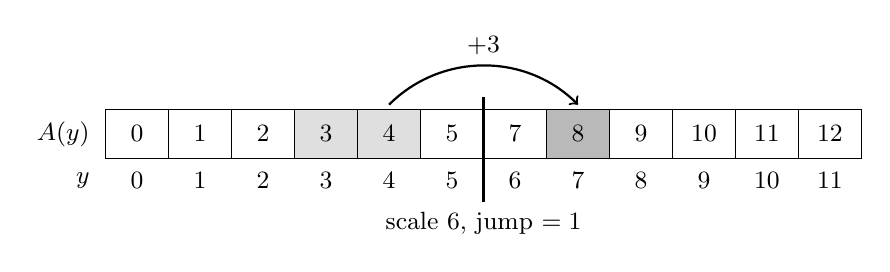
\begin{tikzpicture}[x=0.8cm,y=0.62cm,font=\small]
  \foreach \y in {3,4} \fill[gray!25] (\y,0) rectangle ++(1,1);
  \fill[gray!55] (7,0) rectangle ++(1,1);
  \foreach \y/\v in {0/0,1/1,2/2,3/3,4/4,5/5,6/7,7/8,8/9,9/10,10/11,11/12} {
    \draw (\y,0) rectangle ++(1,1);
    \node at (\y+0.5,0.5) {\v};
    \node at (\y+0.5,-0.45) {\y};
  }
  \node[anchor=east] at (-0.1,0.5) {$\ext A(y)$};
  \node[anchor=east] at (-0.1,-0.45) {$y$};
  \draw[very thick] (6,-0.9) -- (6,1.25);
  \node[anchor=north] at (6,-0.9) {scale $6$, jump $\jump=1$};
  \draw[->,thick] (4.5,1.1) to[bend left=45] node[above,midway] {$+3$} (7.5,1.1);
\end{tikzpicture}
\caption{The carry in \cref{ex:shah}. $A=(6,2):(1,7)$ adds $1$ to every offset beyond the scale
$6$. The two modes of $B$ contribute $4$ and $3$; their sum $7$ lies across the scale, so
$\ext A(7)=8=\ext A(4)+\ext A(3)+\jump$. A rule that composes the modes separately does not see
the carry.}\label{fig:carry}
\end{figure}

\noindent The published conditions for distributing over the modes of $B$ are sufficient
conditions of differing strength. The documentation~\cite{cutedocs} states that composition
distributes when $B$ is injective; \cref{ex:shah} shows that this is false. Cecka~\cite{cecka2026}
requires stride divisibility for every mode and that the modes be \emph{mutually segregated},
$t_ir_i\le r_j$ or $t_jr_j\le r_i$ for all $i\neq j$. If stride divisibility is demanded with
respect to all scales of $A$, this excluded interference in all our tests, and it is far from
necessary (for the $A$ above, $A\circ(2,2):(1,1)=(2,2):(1,1)$ although the two modes coincide).
If each mode is tested only against the scales that it reaches by itself, as in the single-mode
rule, the condition is not sufficient: for $A=(5,2):(1,6)$ and $B=(2,2):(2,4)$ the modes are
segregated and neither reaches the scale $5$, but $\ext A(2+4)=7\neq2+4$.
Shah~\cite[Def.~2.17, Thm.~2.18]{shah2024} requires that the \emph{intervals of definition}
$[r_j,(t_j-1)r_j]\cap[1,P_{m-1})$ of the modes be pairwise disjoint. That condition looks at two
modes at a time, and for three or more modes it is, as printed, not sufficient:

\begin{example}[three modes]\label{ex:three}
$A=(12,2):(1,13)$, $B=(2,2,2):(3,4,6)$. Every mode is admissible in the sense
of~\cite{shah2024}, and the intervals of definition are the single points $3$, $4$ and $6$. No
two of the three strides produce a carry across the scale $12$, but $3+4+6=13$ does:
$\ext A(13)=14$, whereas the concatenation of the per-mode composites, $(2,2,2):(3,4,6)$, gives
$13$.
\end{example}

\noindent The inequality of \cref{def:carryfree} involves all modes at once, and by
\cref{thm:carryfree} it is the exact condition for independent jumps: the modes of $B$ that land
on the same digit of $A$ must fit side by side inside that digit.

\paragraph{Incompleteness: non-monomial strides and non-dividing factors.}
For $t\ge2$ the rule produces only strides of the form $c\cdot d_k$. A composite may need more.

\begin{example}[sum strides]\label{ex:sumstride}
Let $A=\lay{(10,10,10)}{(d_0,d_1,d_2)}$ and $B=10:11$. The digit vector of $11$ is $(1,1,0)$ and
$9\cdot(1,1,0)$ causes no carry, so by \cref{cor:universal} $A\circ B=\lay{10}{(d_0+d_1)}$ for
every choice of strides; but $11$ neither divides nor is divisible by $10$, and the rule rejects
the pair. Similarly $\lay{(11,s)}{(d_0,d_1)}\circ 8:3=\lay{(4,2)}{(3d_0,\;d_0+d_1)}$ for all
$d_0,d_1$ and all $s\ge 2$: the refinement $(4,2):(3,12)$ of $8:3$ has stride digits $(3,0)$ and
$(1,1)$, and $3\cdot(3,0)+1\cdot(1,1)=(10,1)$ does not overflow the digit of size $11$.
\end{example}

The second example shows that even the single-term question ``when is $x\mapsto\floor{rx/P}$ a
layout function on $\rng t$?'' has a non-obvious answer; it is recorded in \cref{prop:dilated}.

\begin{proposition}[one dilated floor term]\label{prop:dilated}
Let $1\le\rho<q$ be coprime, $u=\ceil{q/\rho}$ and $e=u\rho-q$. The function
$x\mapsto\floor{\rho x/q}$ on $\rng t$ is a layout function if and only if $t\le u$, or $u\mid t$
and either $e=0$ or $t\le(\ceil{\rho/e}-1)\,u$. In the second case it equals $x\mapsto\floor{x/u}$.
\end{proposition}
\begin{proof}
The function is $0$ on $\rng u$ and increases by one at the points
$n_j=\ceil{jq/\rho}=ju-\floor{je/\rho}$, $j\ge1$. If $t\le u$ it vanishes. If $e=0$ then
$\rho\mid q$, so $\rho=1$, and the function is $x\mapsto\floor{x/u}$, a layout function on
$\rng t$ iff $u\mid t$ (\cref{thm:spectrum}(a)). Let $e\ge1$ and $J=\ceil{\rho/e}$. Since
$e<\rho$ we have $(J-1)e<\rho\le Je<2\rho$, so $n_j=ju$ for $j<J$ and $n_J=Ju-1$: the function
agrees with $\floor{x/u}$ below $Ju-1$ and exceeds it by $1$ there. Hence for $u<t\le Ju-1$ it
is a layout function iff $u\mid t$, i.e.\ iff $t\in\{2u,\dots,(J-1)u\}$; and for $t\ge Ju$ its
floor spectrum contains $u$ and $Ju-1$, which is not a multiple of $u$, so by
\cref{thm:spectrum}(a) it is not a layout function.
\end{proof}

\subsection{Laws}\label{sec:laws}

\begin{proposition}\label{prop:laws}
\begin{enumerate}[label=(\alph*),itemsep=1pt]
\item \emph{Identity.} $A\circ(\lay N1)$ is $A$ truncated or extended to size $N$, when that is
 a layout; and $(\lay N1)\circ B=B$.
\item \emph{Reshape.} For a column-major $B$ with shape $T$ (so $\bnd B$ is the identity),
 $A\circ B$ exists if and only if $\spec(\ext A|_{\rng{|T|}})\cup\Sc(T)\cup\{|T|\}$ is a chain
 under divisibility.
\item \emph{Distributivity.} $A\circ(B_0,\dots,B_{n-1})=(A\circ B_0,\dots,A\circ B_{n-1})$ holds
 exactly when the right-hand side exists and the non-interference condition of
 \cref{thm:exact}(iii) is satisfied.
\item \emph{Associativity.} Let $C$ be $\N$-valued with $\bnd C(\rng{|C|})\subseteq\rng{|B|}$, and
 suppose $A\circ B$ and $B\circ C$ exist, $B\circ C$ being represented as in \cref{thm:exact}
 (each $R_j$ coalesced). If $(A\circ B)\circ C$ and $A\circ(B\circ C)$ both
 exist, they have the same function. If $A\circ(B\circ C)$ exists then so does
 $(A\circ B)\circ C$. The converse can fail.
\item \emph{Additivity in $A$.} If $A_1,A_2$ have the same shape then
 $(A_1+A_2)\circ B=A_1\circ B+A_2\circ B$ over any refinement over which both sides exist.
\end{enumerate}
\end{proposition}
\begin{proof}
(a) and (e) are immediate. (b) is \cref{thm:exact}(iv) with $g=\ext A|_{\rng{|T|}}$: the set is
a chain iff $g$ is a layout function (\cref{thm:spectrum}(a)) whose spectrum is compatible with
$\Sc(T)$. (c) is \cref{thm:exact}. (d): by the in-bounds hypothesis the extended function of the
layout $A\circ B$ agrees with $\ext A\circ\bnd B$ on the values of $C$, so each bracketing, if it
exists, represents $h=\ext A\circ\bnd B\circ\bnd C$. By \cref{thm:exact}, $(A\circ B)\circ C$
exists iff $h$ is additive over a by-mode refinement of the shape of $C$, whereas
$A\circ(B\circ C)$ exists iff $h$ is additive over a by-mode refinement of the shape of the
layout $B\circ C$, which itself refines the shape of $C$. This gives the implication, and shows
why the converse may fail: the intermediate layout $B\circ C$ may have scales that $h$ does not
tolerate. (The representative matters: for $A=(2,3):(0,1)$ and $B=C=6:1$, composing $A$ with
$B\circ C=6:1$ works, whereas the finer layout $(3,2):(1,3)$ with the same function would not
do.)
\end{proof}

\begin{example}[associativity]\label{ex:assoc}
Let $A=(12,3):(0,1)$, $B=(2,2,3,3):(1,6,2,12)$ and $C=6:7$; the values of $C$ lie in
$\rng{36}=\rng{|B|}$. Here $\bnd B$ permutes each block of $12$ consecutive numbers, so
$A\circ B$ has function $\floor{x/12}$, and $(A\circ B)\circ C=(2,3):(0,1)$ with function
$h(x)=\floor{7x/12}=\floor{x/2}$ on $\rng6$. But $B\circ C=(3,2):(9,17)$ has the scale $3$,
which is incomparable with the scale $2$ of $h$, so $A\circ(B\circ C)$ does not exist. Without
the in-bounds hypothesis even the functions can differ~\cite{cecka2026}:
$\bigl((5,3):(1,7)\circ4:1\bigr)\circ2:5=2:5$ but $(5,3):(1,7)\circ\bigl(4:1\circ2:5\bigr)=2:7$.
\end{example}
